% Section content template for individual Educative lessons
% This file contains the actual content for a specific section
% Generated from Educative API section content

% Section: Class Diagram for the Library Management System
% Section ID: 4823331759194112
% Section Slug: class-diagram-for-the-library-management-system
% Generated: 2025-12-11T15:13:16.598007

Here, we'll create the class diagram for our system based on the previously gathered requirements. In the class diagram, we will first design/create the classes, abstract classes, and interfaces for the system, and then we'll identify the relationship between classes in accordance with all requirements of the library management system.

\subsection{Components of a library management system}\label{JAUOBQIi_DfVKg7jmDVBk}
\\
In this section, we will define the classes for LMS. Following the bottom-up approach for designing a class diagram, we'll first create the classes of small components. After that, we will integrate those components and create the class diagram for the library management system.

\subsubsection{Book and book item}\label{YaHWa-Ru4MUTFL0wY4OEp}
\\
The \texttt{Book} class represents the conceptual essence of a book. This includes metadata or descriptive information about a book that isn't specific to any physical copy. It serves as a blueprint that captures the shared attributes of all instances or copies of the book, whether in the world or within the library's collection.
\\
The \texttt{BookItem} class, in contrast, represents a specific physical or digital instance of a \texttt{Book} in the library's collection. Rather than extending the \texttt{Book}, it has a composition relationship with it, meaning each \texttt{BookItem} is tightly associated with a \texttt{Book}. All corresponding \texttt{BookItem} instances must also be deleted if a \texttt{Book} is deleted. The
\texttt{BookItem} class handles the properties and behaviors associated with individual copies that patrons can borrow, reserve, or reference within the library. Each
\texttt{BookItem} has unique attributes to manage and track its status within the library system. The
UML representation of \texttt{Book} and \texttt{BookItem} is shown in the class diagram below:

\begin{figure}[htbp]
 \centering
 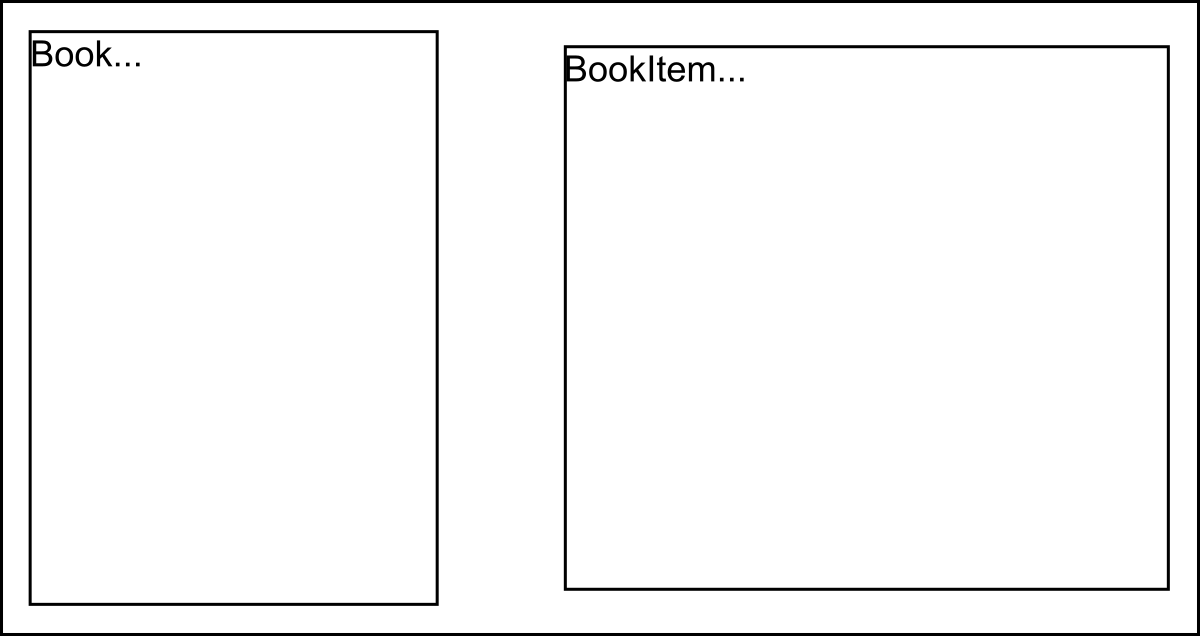
\includegraphics[width=0.5\textwidth]{Images/chapter_9/section_4823331759194112/6045313755381760.png}
 \caption{The class diagram of the Book and BookItem classes}
\end{figure}

\textbf{R3:} Every book should have an associated \#key\# ISBN: International Standard Book Number \#key\#, title, author name, subject, and publication date.
\\
\textbf{R4:} Multiple copies of the book can be made, and each copy will be recognized as a book item.

\subsubsection{Rack}\label{he706RE4-ZG1bz71Kj8x0}
\\
We have seen a complex object, \texttt{Rack}, that was defined in the \texttt{BookItem} class. Now , we are going to create a \texttt{Rack} class. This class is used to identify the physical location of any book item in the library. Every rack has a specific rack number and a location identifier to represent the location of the book item in the library. The visual representation of the class is as follows:

\begin{figure}[htbp]
 \centering
 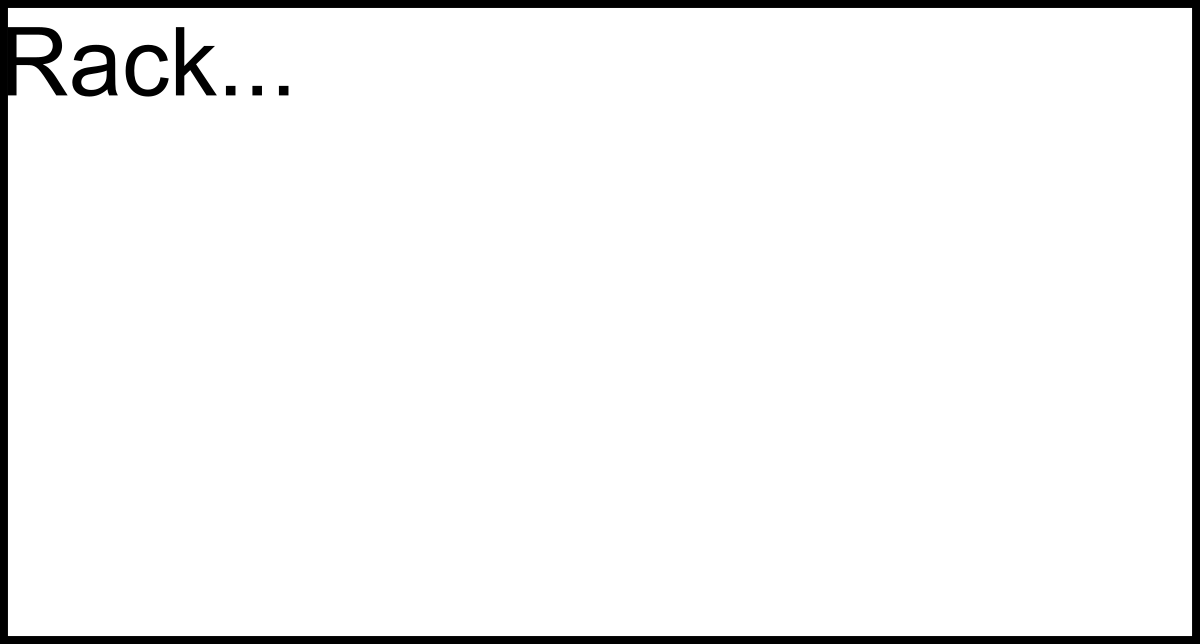
\includegraphics[width=0.5\textwidth]{Images/chapter_9/section_4823331759194112/5182924108595200.png}
 \caption{The class diagram of the Rack class}
\end{figure}

\textbf{R2:} Every book is supposed to have a unique identification number and other details, including a rack number, to help locate it physically.

\subsubsection{Person and author}\label{7WY0pQMv4IW5dcsZzqUEA}
\\
The \texttt{Person} class stores information related to a person, such as a name, email, phone number, etc. It also contains an object of the \texttt{Address} class to specify the person's address.
\\
There is also a class named \texttt{Author} that stores the author's data, such as the author's name and description. The author's information is also used in the \texttt{Book} class.
\\
The representation of both classes is as follows:

\begin{figure}[htbp]
 \centering
 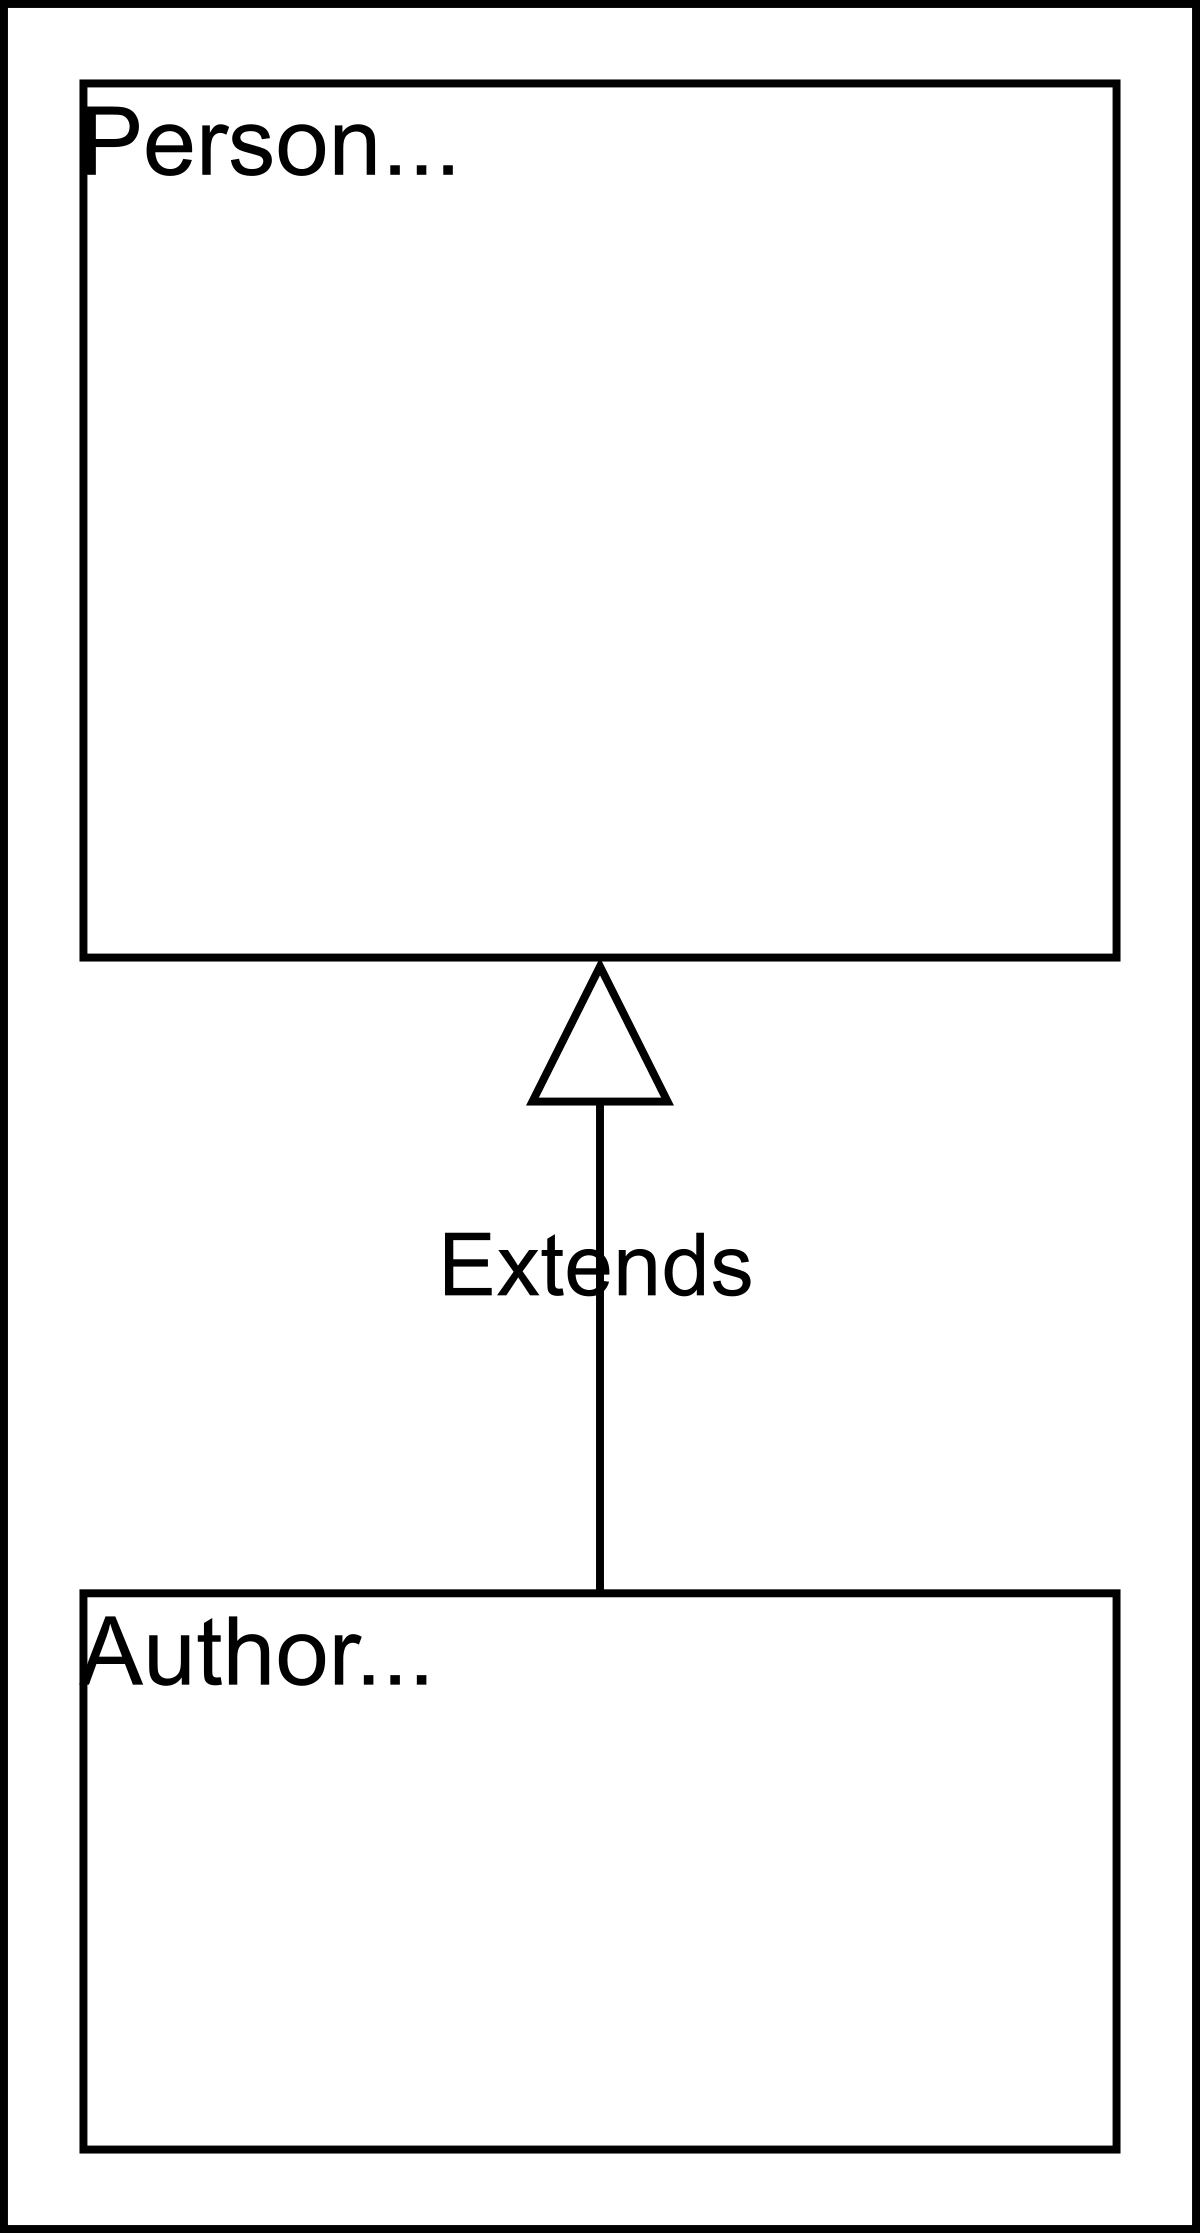
\includegraphics[width=0.5\textwidth]{Images/chapter_9/section_4823331759194112/4563004562866176.png}
 \caption{The class diagram of the Person and Author classes}
\end{figure}

\subsubsection{User, librarian, and library member}\label{IvphcDXG3JfvlGrZDXvLi}
\\
\texttt{User} is an abstract class that represents the LMS system users. There are two types of users: librarians and library members.
\\
The \texttt{Librarian} class is a derived class of the \texttt{User} class. It is responsible for adding new book items and blocking or unblocking any library member.
\\
Similar to the \texttt{Librarian} class, the \texttt{Member} class extends the \texttt{User} class. The variable \texttt{totalBooksCheckedout} stores the number of books a member has already checked out. A member can reserve a book, return a book, or renew an already reserved book.
\\
Since the \texttt{Librarian} and \texttt{Member} classes extend the \texttt{User} class, their class diagram representation would be as follows:

\begin{figure}[htbp]
 \centering
 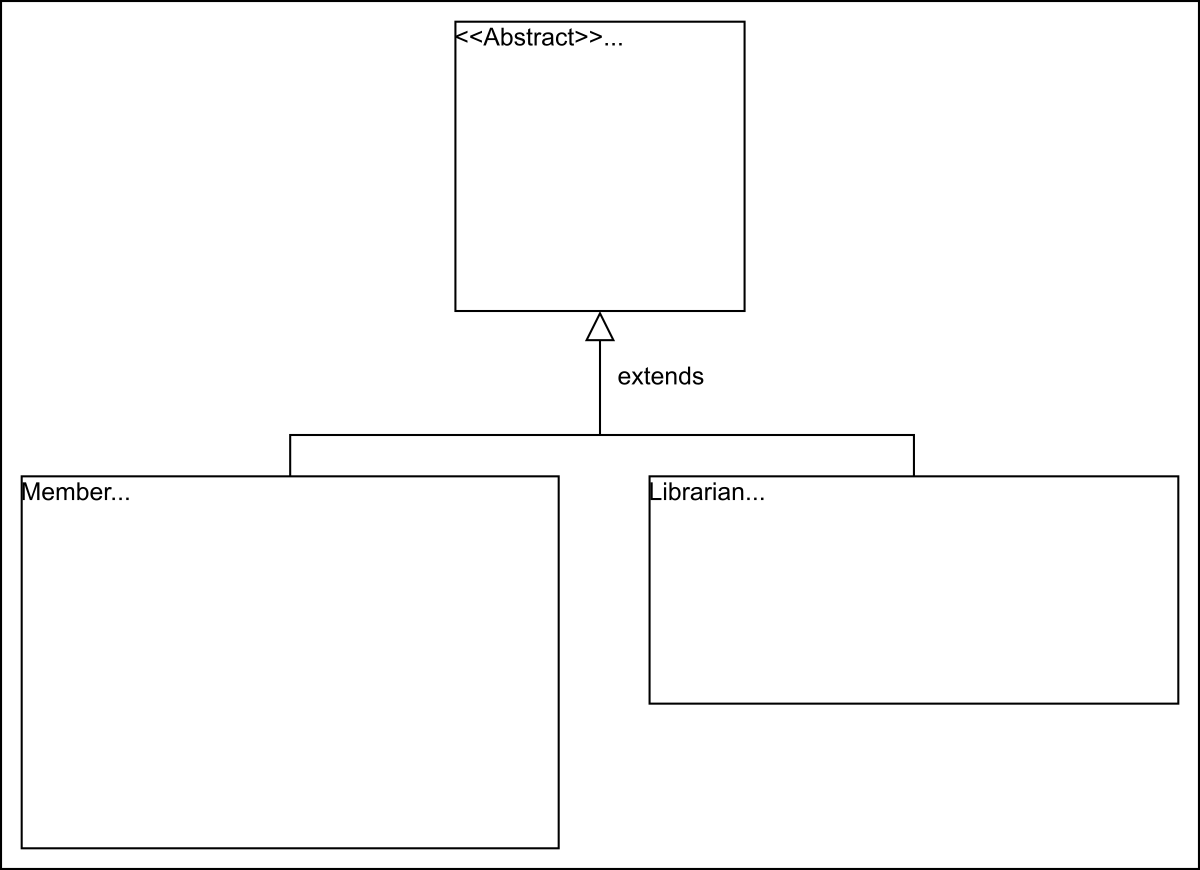
\includegraphics[width=0.5\textwidth]{Images/chapter_9/section_4823331759194112/5081485095993344.png}
 \caption{The class diagram of the User, Librarian, and Member classes}
\end{figure}

\textbf{R5:} There can be two types of users: the librarian and the members.
\\
\textbf{R11:} The system should allow the user to renew the reserved book.

\subsubsection{Library card}\label{YmCCH32z-2jf5IC4Z6dV4}
\\
To manage each user's library card information, we have a \texttt{LibraryCard} class. Each library card has an identification number, issue date, and information on whether or not it is active. The class representation of the \texttt{LibraryCard} class is as follows:

\begin{figure}[htbp]
 \centering
 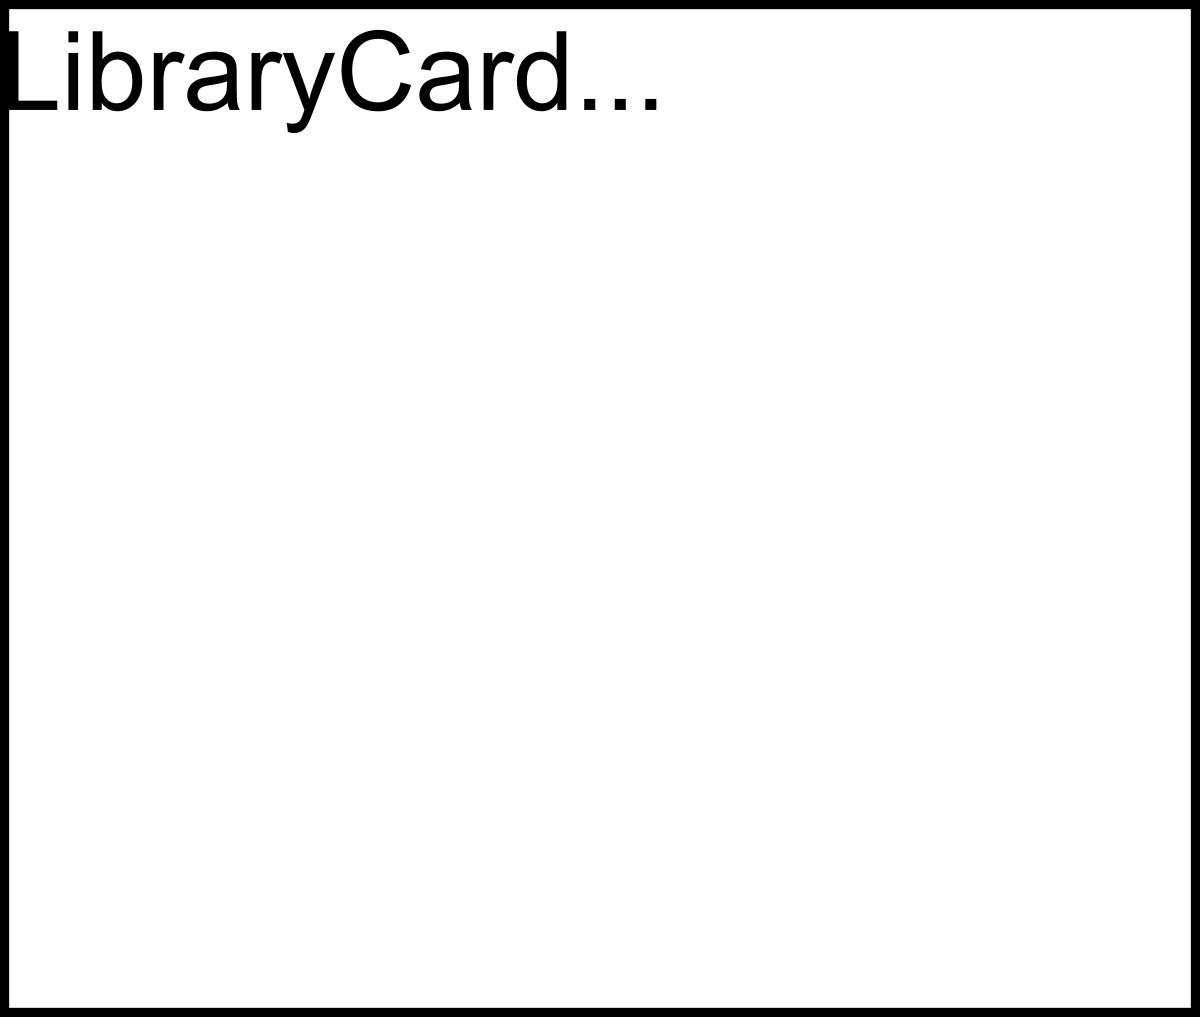
\includegraphics[width=0.5\textwidth]{Images/chapter_9/section_4823331759194112/5293705944891392.png}
 \caption{The class diagram of the LibraryCard class}
\end{figure}

\textbf{R6:} Every user must have a library card with a unique card number.

\subsubsection{Book reservation}\label{KiBO4XKPxRKzIgJ9J6XVu}
\\
Book reservation is one of the library management system's most important requirements. To fulfill this functionality, we have a class named \texttt{BookReservation}. This class is responsible for managing the book reservation status of book items.
\\
The UML representation of the class is shown below:

\begin{figure}[htbp]
 \centering
 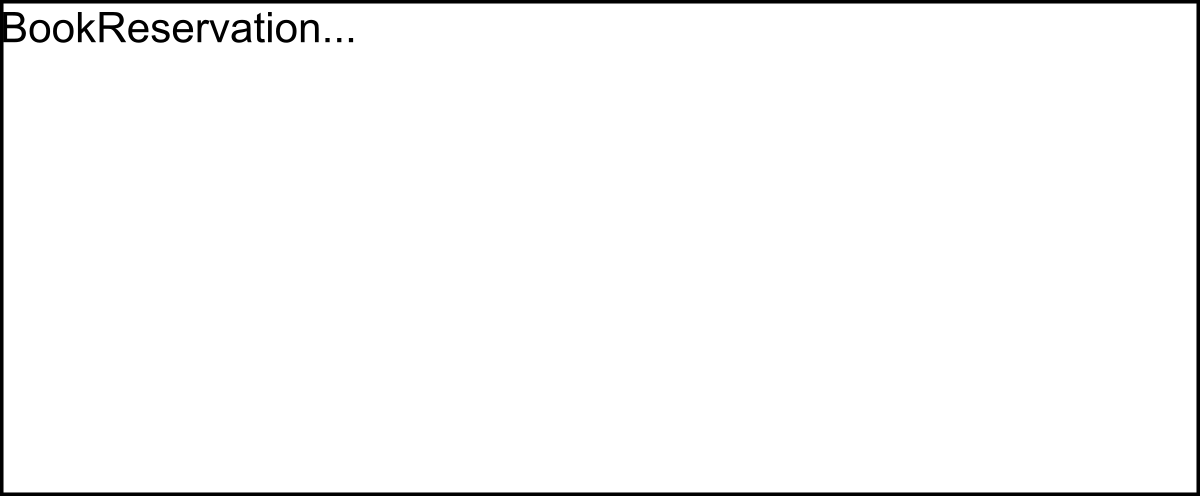
\includegraphics[width=0.5\textwidth]{Images/chapter_9/section_4823331759194112/6257240183144448.png}
 \caption{The class diagram of the BookReservation class}
\end{figure}

\textbf{R10:} The system should be able to record who issued or reserved a particular book and on which date.

\subsubsection{Book lending}\label{stpOTD01LbFXMxI6w7kp2}
\\
Similar to book reservations, book lending is also part of the system since the \texttt{BookLending} class manages the process of checking out book items. This class handles or processes information like the book lending date, due date, return date, etc.
\\
Here is what the class definition looks like:

\begin{figure}[htbp]
 \centering
 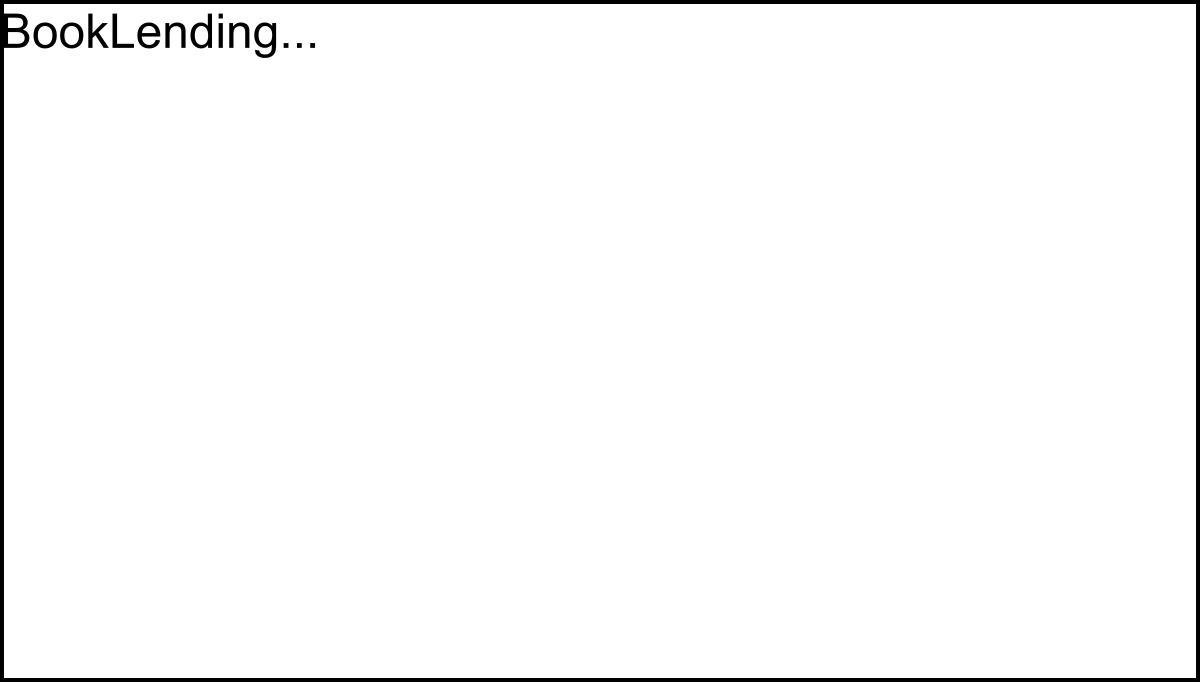
\includegraphics[width=0.5\textwidth]{Images/chapter_9/section_4823331759194112/4851403837407232.png}
 \caption{The class diagram of the BookLending class}
\end{figure}

\subsubsection{Notification}\label{BQtZ_SI28rM8oQKwwiUXe}
\\
\texttt{Notification} is an abstract class. If the book is not returned within the due date, the class notification is responsible for informing library members by sending a notification. Every notification has an ID, creation date, and content. The notification can be either a \emph{postal notification} or an \emph{email notification}.
\\
The \texttt{PostalNotification} class requires the address of the library member to send a notification, while \texttt{EmailNotification} needs the email address of the library member to send a notification.
\\
The relationship diagram of these classes is shown below:

\begin{figure}[htbp]
 \centering
 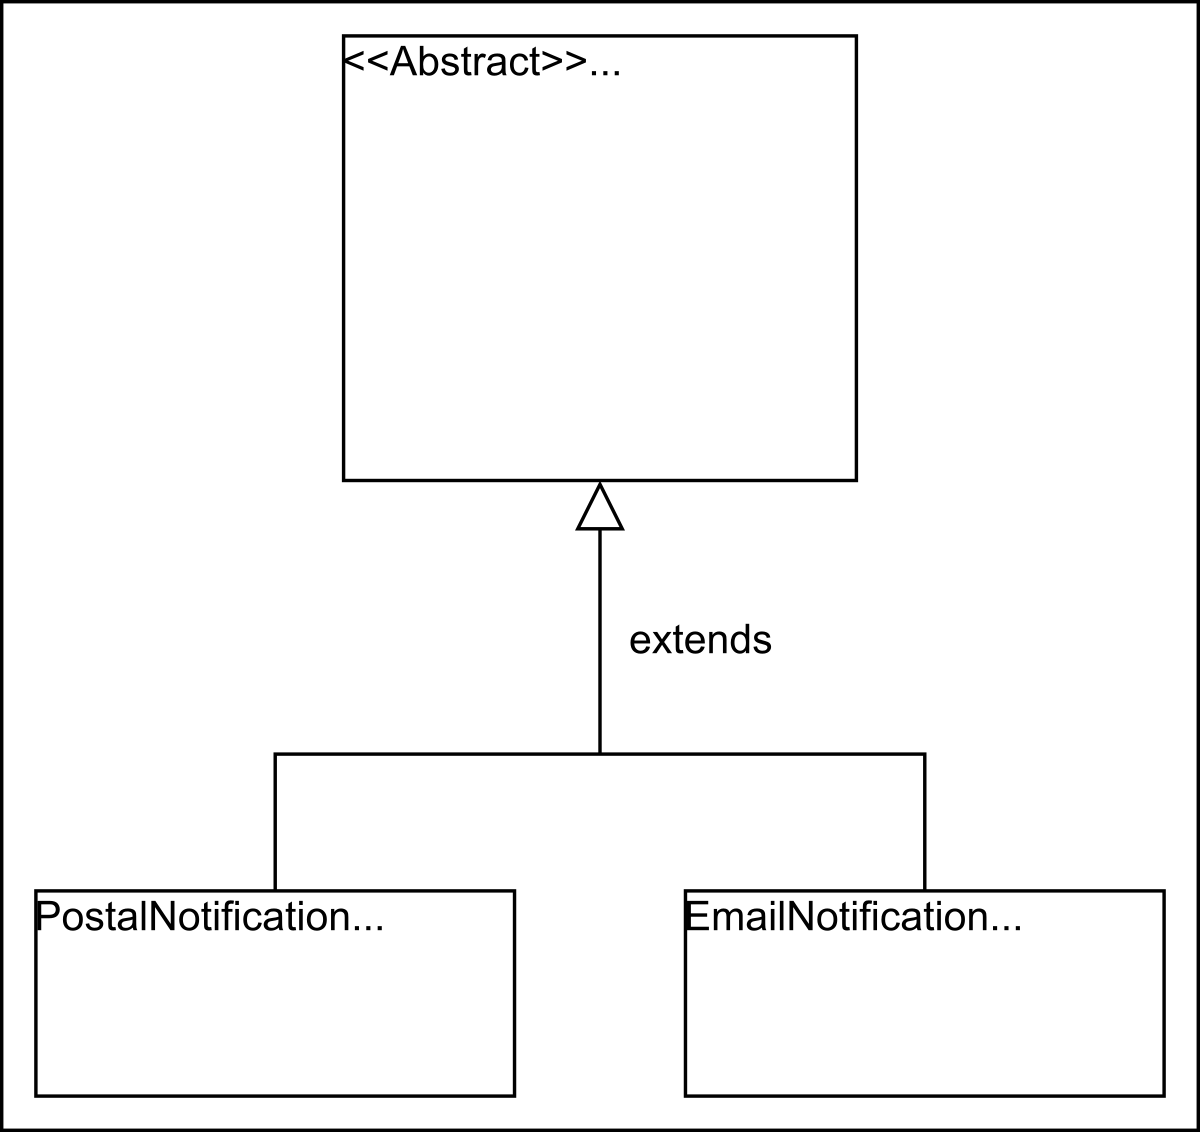
\includegraphics[width=0.5\textwidth]{Images/chapter_9/section_4823331759194112/6698623016632320.png}
 \caption{The class diagram of the Notification, PostalNotification, and EmailNotification classes}
\end{figure}

\textbf{R12:} The system should notify if the book is not returned within the due date.

\subsubsection{Search and catalog}\label{NkCWtMGTbWNJFk4MxYwVm}
\\
Search is one of the most important functionalities of the system. \texttt{Search} is the interface that allows the user to search for any book and return the list of books upon searching by any of the following methods:

\begin{itemize}
\item
\protect\phantomsection\label{cWavjsR3N2RpmB0wRy0W_}
Search for a book by its title.
\item
\protect\phantomsection\label{VE_AbtFSrNVmCeuKL8d3-}
Search for a book by its author's name.
\item
\protect\phantomsection\label{i-I8q0bXi5MlMdlAOYlY4}
Search for a book by itssubject.
\item
\protect\phantomsection\label{4jh08Psqmz_d4o2xsaaKH}
Search for a book by its publication date.
\end{itemize}
\\
\texttt{Catalog} is a class where the search functionality is implemented. In each catalog, the books are sorted according to one search technique, i.e., based on the book's title, author, subject, or publication date.
\\
The following UML diagram shows this relationship:

\begin{figure}[htbp]
 \centering
 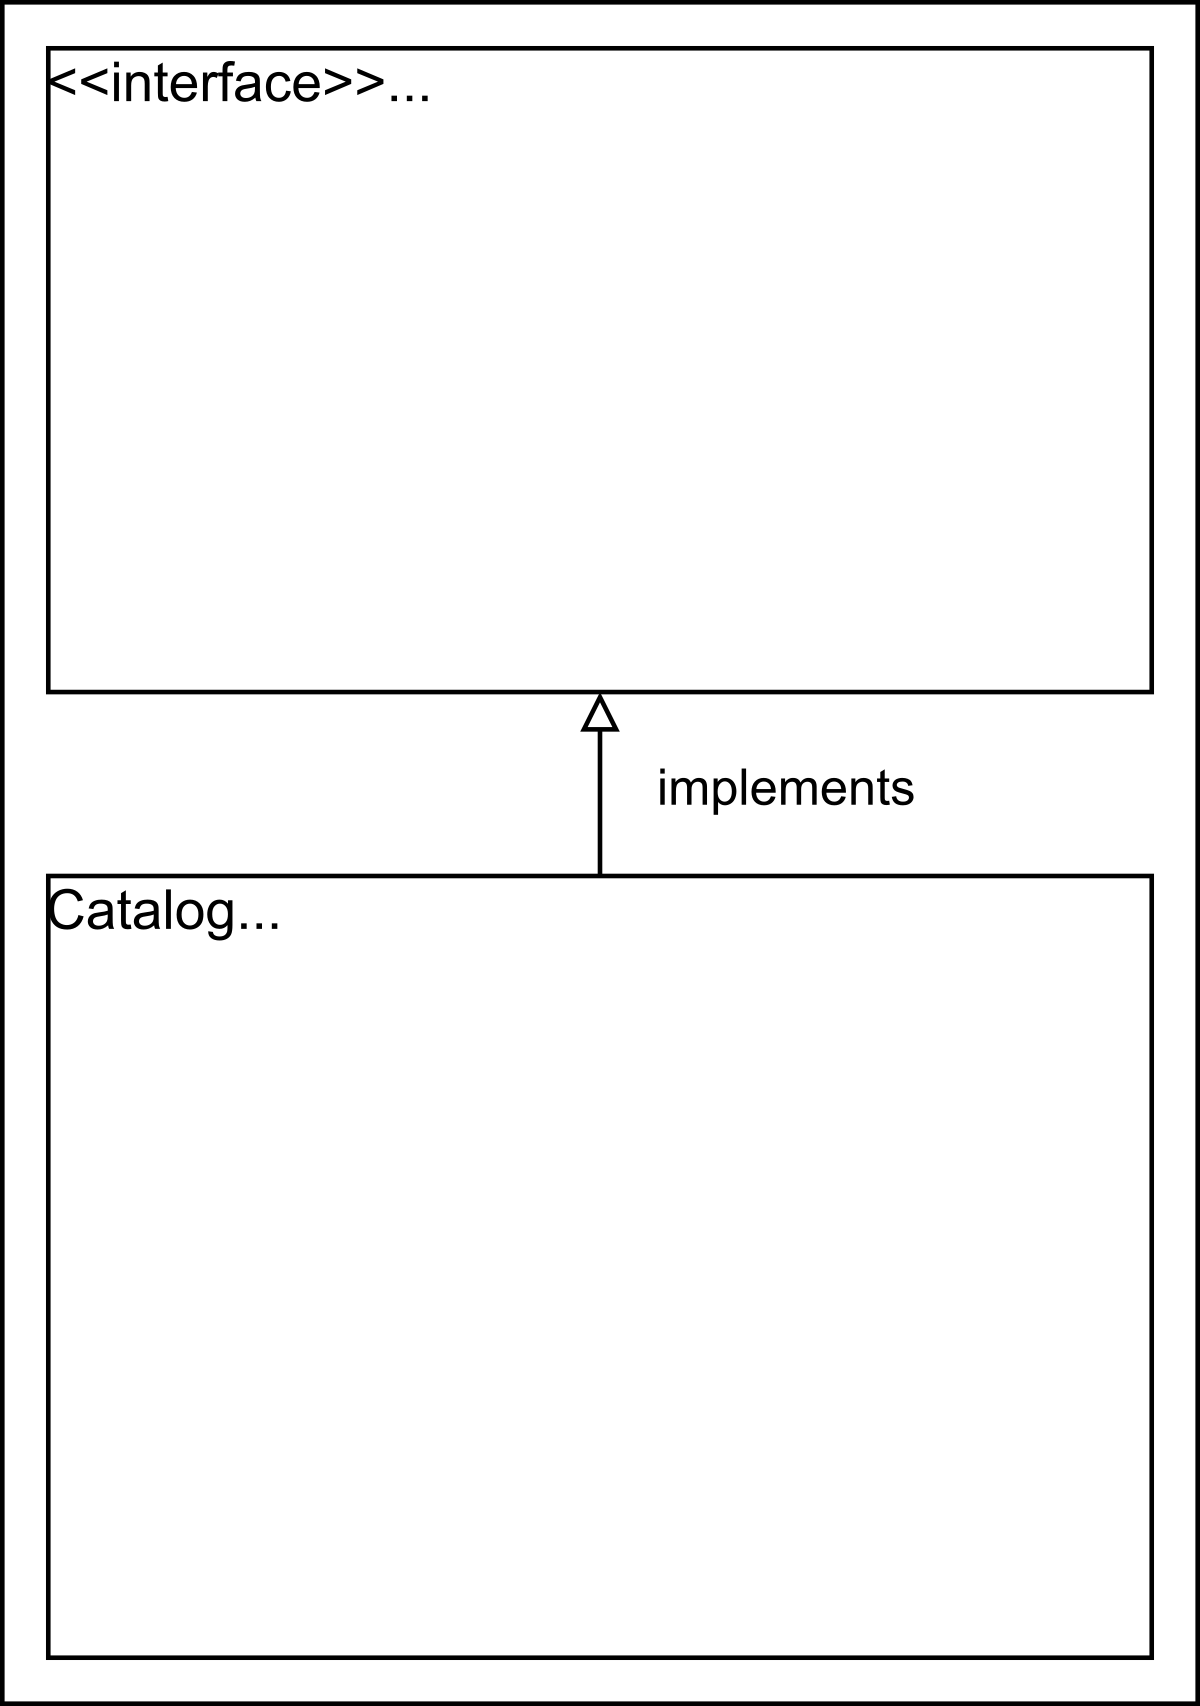
\includegraphics[width=0.5\textwidth]{Images/chapter_9/section_4823331759194112/6057625600131072.png}
 \caption{The class diagram of the Search and Catalog classes}
\end{figure}

\textbf{R14:} The system should allow users to search for a book by title, author name, subject, or publication date.

\subsubsection{Library}\label{g8J5oylLx2FdIkZRWTTCD}
\\
The \texttt{Library} class is the base class of the system, which is used to represent the library. It is a central part of the organization. This class consists of two members: name and \texttt{Address}. The string type name stores the library's \texttt{name}, while the complex object \texttt{Address} stores the library's complete address location. The UML representation of the \texttt{Library} class is as follows:

\begin{figure}[htbp]
 \centering
 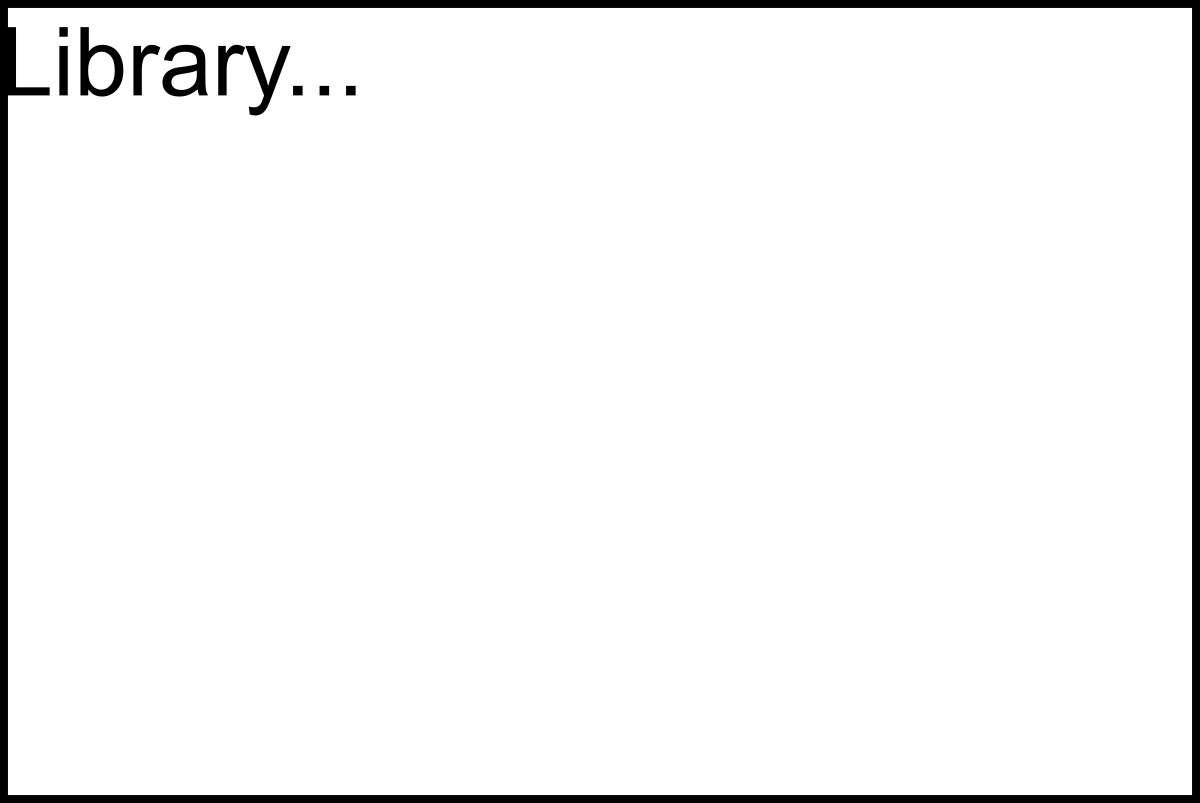
\includegraphics[width=0.5\textwidth]{Images/chapter_9/section_4823331759194112/5411623533805568.png}
 \caption{The class diagram of the Library class}
\end{figure}

\subsubsection{Enumerations}\label{7ryiXEenoB1Cm4-F-b01l}
\\
Enumeration is generally a data type in which only a specific set of constants can be stored. The following is a list of enumerations required in LMS:
\\
\texttt{BookFormat}: A book can only be of one of the specified formats. It can be a hardcover, paperback, audiobook, e-book, newspaper, magazine, or journal.
\\
\texttt{BookStatus}: The book status describes the status of the particular book item for the user, whether it is available, reserved, loaned, or lost.
\\
\texttt{ReservationStatus}: This tells about the reservation state of any book item, whether in a waiting state, pending state, canceled state, or none of them.
\\
\texttt{AccountStatus}: The account status tells about the user account status, whether it is active, closed, canceled, blocklisted, or none.

\begin{figure}[htbp]
 \centering
 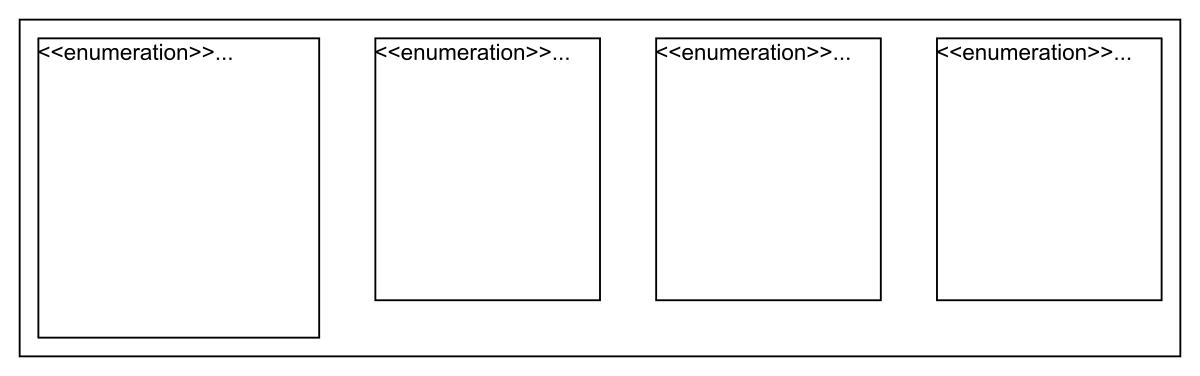
\includegraphics[width=0.5\textwidth]{Images/chapter_9/section_4823331759194112/4605724781838336.png}
 \caption{Enums in the library management system}
\end{figure}

\subsubsection{Custom data type}\label{t2sP-2giPd1XhSaFWsMuD}
\\
The \texttt{Address} is a custom data type that stores the address of a library and its users.

\begin{figure}[htbp]
 \centering
 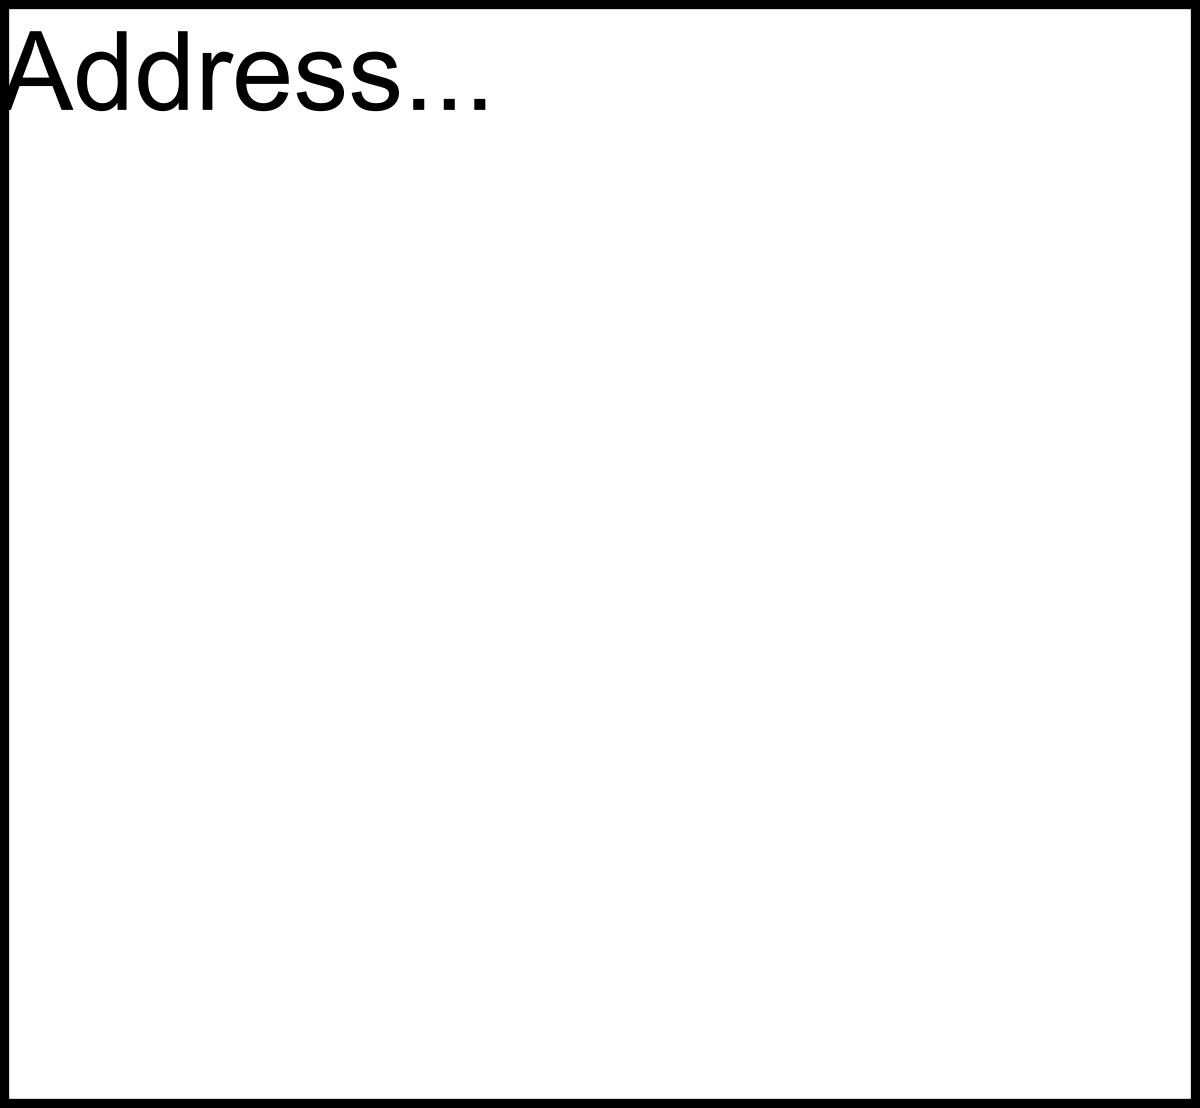
\includegraphics[width=0.5\textwidth]{Images/chapter_9/section_4823331759194112/5838664733294592.png}
 \caption{Class diagram of the Address custom data type}
\end{figure}

\subsection{Relationship between the classes}\label{9oMLdXziMepI7oI4BO2Ms}
\\
Now, we will discuss the relationships between the classes we defined above in our library management system.

\subsubsection{Association}\label{SZ-C1YsLzfbaCLUX0xA0T}
\\
The class diagram has the following association relationships:
\\
\paragraph{One-way association}\label{CKgtTrk8oB_5KRfW-QQih}

\begin{itemize}
\item
\protect\phantomsection\label{fkLAU5K-SiT0OFkKfbu5h}
The \texttt{User} has a one-way association with \texttt{BookItem} and \texttt{BookReservation}.
\item
\protect\phantomsection\label{Mt78Ajscq9zgUaf1zwMyU}
Both \texttt{BookReservation} and \texttt{BookLending} have a one-way association with the \texttt{BookItem}.
\end{itemize}

\begin{figure}[htbp]
 \centering
 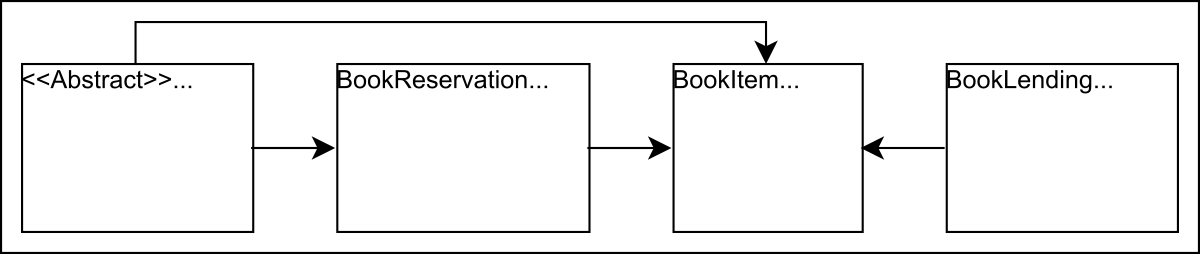
\includegraphics[width=0.5\textwidth]{Images/chapter_9/section_4823331759194112/6199370795188224.png}
 \caption{The one-way association relationship between the classes}
\end{figure}

\paragraph{Two-way association}\label{TupnrQoLkEYbhrI_l-TZG}

\begin{itemize}
\item
\protect\phantomsection\label{UKahIU7l1_crYFiY_Gzp4}
\texttt{Author} has a two-way association with \texttt{Book}.
\item
\protect\phantomsection\label{UEsY39rQwMfqEUR2flE0U}
Both \texttt{Rack} and \texttt{Librarian} have a two-way association with \texttt{BookItem}.
\item
\protect\phantomsection\label{C_nHr7Yb8vi6y0xeFu61L}
The \texttt{Notification} has a two-way association with \texttt{BookLending} and \texttt{BookReservation}.
\item
\protect\phantomsection\label{dj5vjMZP1sHiaWMsJKfs_}
The \texttt{BookLending} has a two-way association with \texttt{BookReservation} and \texttt{User}.
\end{itemize}

\begin{figure}[htbp]
 \centering
 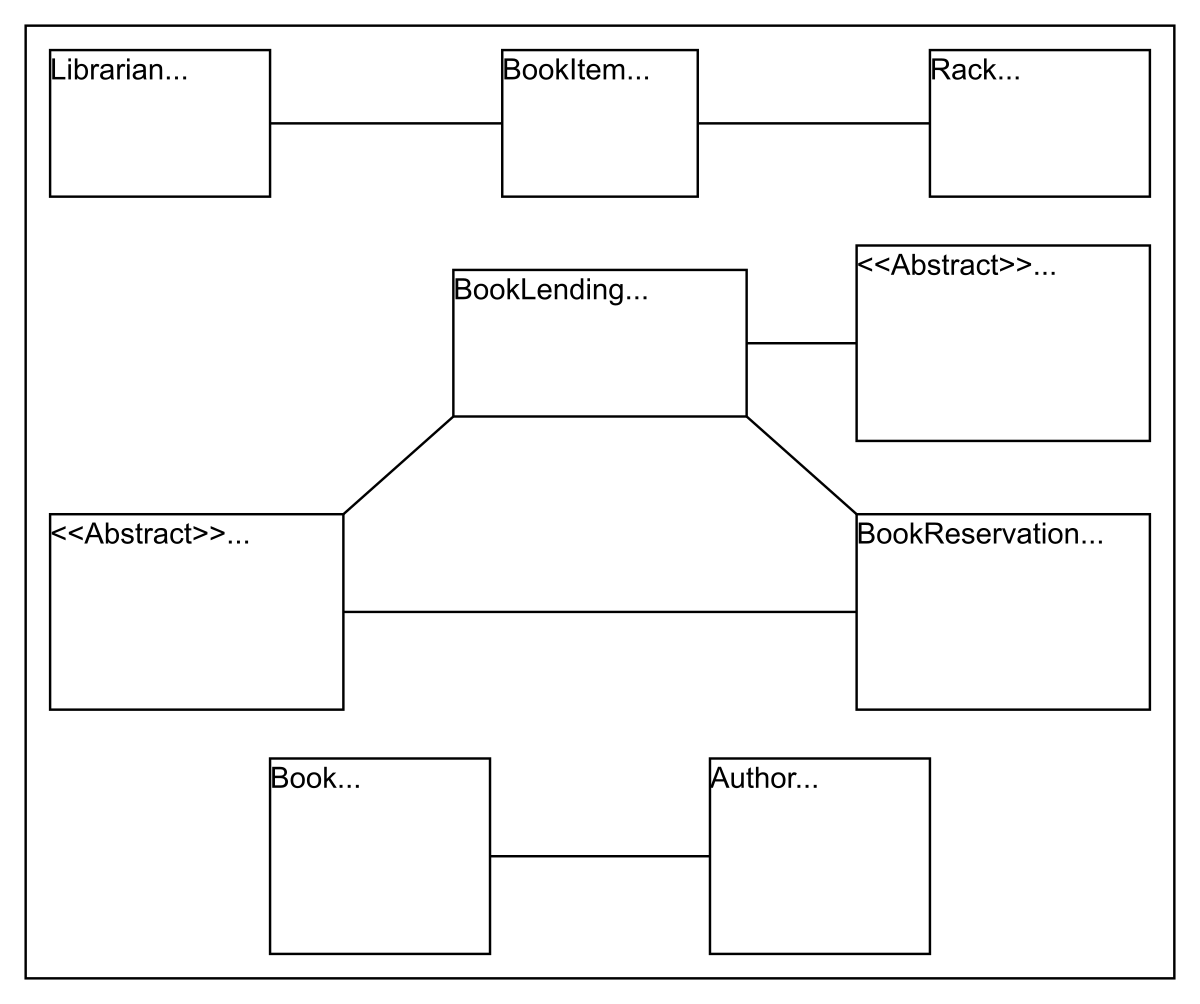
\includegraphics[width=0.5\textwidth]{Images/chapter_9/section_4823331759194112/5805872737288192.png}
 \caption{The two-way association relationship between the classes}
\end{figure}

\subsubsection{Composition}\label{PjvQgVZ1S_TA_oStj1z8s}

\begin{itemize}
\item
\protect\phantomsection\label{biOg8Qp_4TsWCaawFadZ5}
\texttt{Library} is composed of \texttt{BookItem}.
\item
\protect\phantomsection\label{IgkwIATbaEPgQQKlxvfet}
\texttt{User} is composed of \texttt{LibraryCard}.
\item
\protect\phantomsection\label{nM9_FegCaVJsd_mjZs1vF}
\texttt{Book} is composed of \texttt{BookItem}.
\end{itemize}

\begin{figure}[htbp]
 \centering
 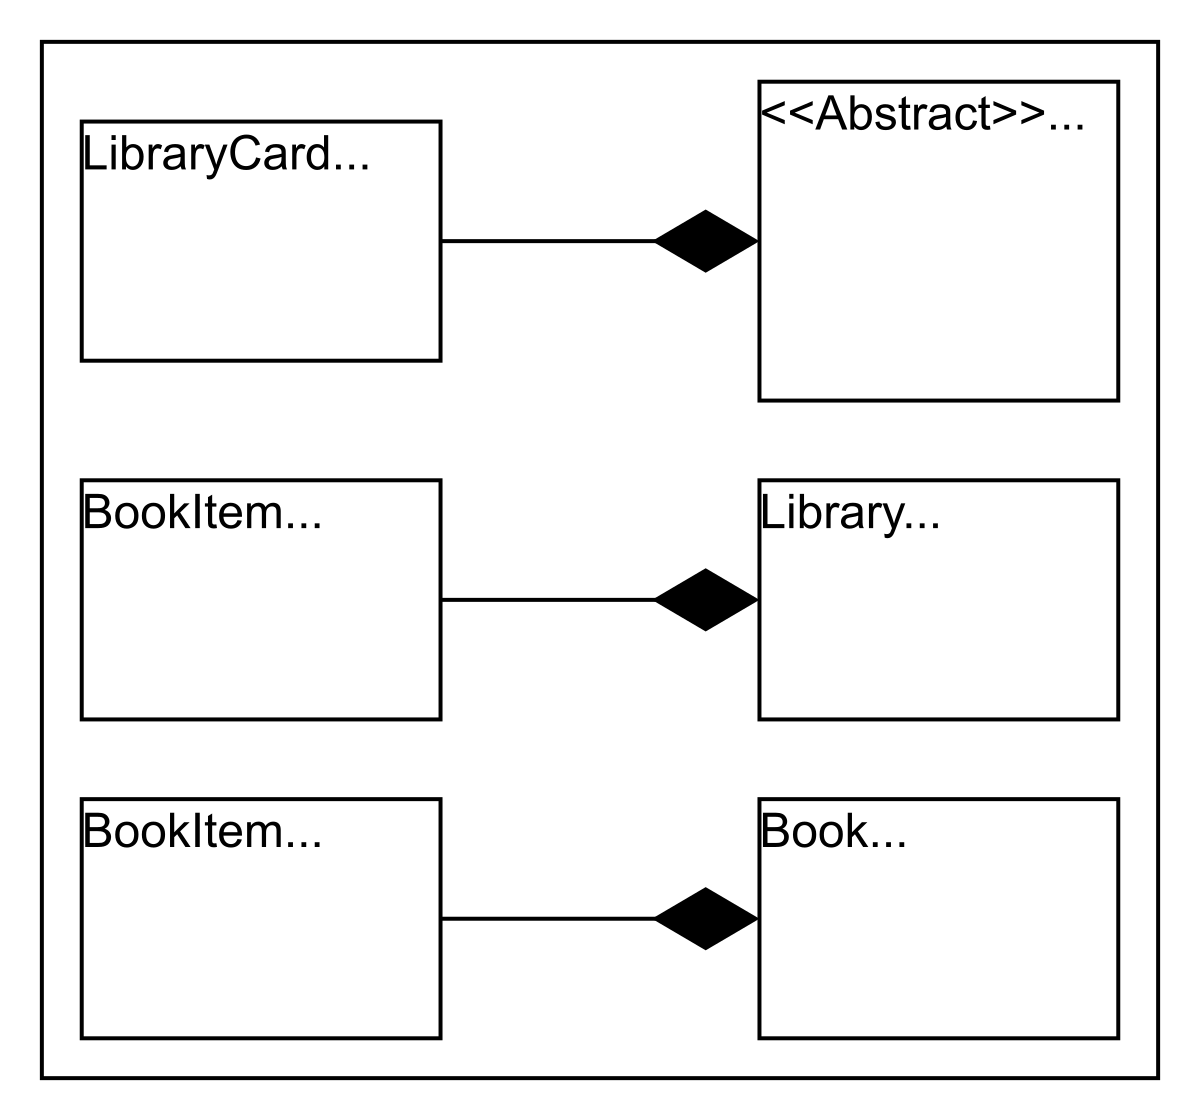
\includegraphics[width=0.5\textwidth]{Images/chapter_9/section_4823331759194112/5689720947212288.png}
 \caption{The composition relationship between the classes}
\end{figure}

\subsubsection{Aggregation}\label{MpoEZsVElp8OVKUfMkK_Y}

\begin{itemize}
\item
\protect\phantomsection\label{CSoomJ9WxLntBkF56FGnr}
The \texttt{Catalog} class contains the \texttt{Book} class.
\end{itemize}

\begin{figure}[htbp]
 \centering
 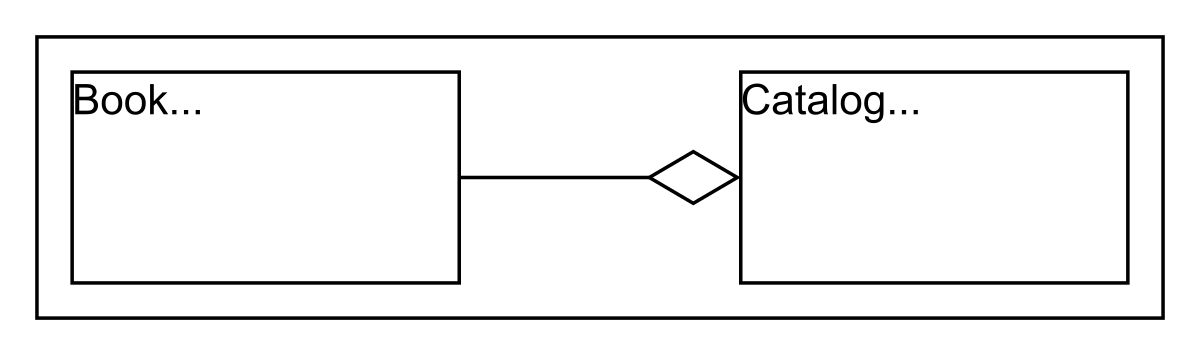
\includegraphics[width=0.5\textwidth]{Images/chapter_9/section_4823331759194112/6481425257594880.png}
 \caption{The aggregation relationship between the classes}
\end{figure}

\subsubsection{Inheritance}\label{nitAA55uozDxbLp-u945B}
\\
The following classes show an inheritance relationship:

\begin{itemize}
\item
\protect\phantomsection\label{p9PNBidGVl70shfUaIB4f}
Both \texttt{Librarian} and \texttt{Member} classes extend the \texttt{User} class.
\item
\protect\phantomsection\label{G_OkULC1jofOFgimVlgsV}
Both \texttt{EmailNotification} and \texttt{PostalNotification} classes extend the \texttt{Notification} class.
\item
\protect\phantomsection\label{l9NW9IZ1bZkvGyODX8aJn}
The \texttt{Catalog} class implements the \texttt{Search} interface.
\end{itemize}
\begin{quote}
\textbf{Note:} We have already discussed the inheritance relationship between classes in the component section above one by one.
\end{quote}
\subsection{Class diagram of the library management system}\label{ZMh0asTYHa8mkNjmC5LA4}
\\
This section outlines the multiplicity (cardinality) relationships between the main classes in our Library Management system. We explain the allowed number of instances on each side for each relationship and the real-world or design rationale behind the connection. Understanding these relationships is key to modeling how different entities interact and collaborate to support key workflows in the system.

\begin{center}
\begin{tabular}{|p{0.18\linewidth}|p{0.18\linewidth}|p{0.12\linewidth}|p{0.45\linewidth}|}
\hline
\textbf{Source} & \textbf{Target} & \textbf{Multiplicity} & \textbf{Reason} \\
\hline
Library & BookItem & 1 -- 1..* & A library must have at least one book item, and can have many. \\
\hline
Rack & BookItem & 1 -- 0..* & Each rack may have zero or many book items. \\
\hline
Book & BookItem & 1 -- 1..* & Each book item is a copy of exactly one book. \\
\hline
Book & Author & 1..* -- 1..* & Every book has at least one author (possibly more). Similarly, every author can write one or many books. \\
\hline
User & LibraryCard & 1 -- 1 & Each user has one library card. \\
\hline
User & BookLending & 1 -- 0..* & A user can have zero or more lending records. \\
\hline
BookReservation & BookItem & 1 -- 0..1 & Each reservation is for one specific book item. \\
\hline
Catalog & Book & 1 -- 1..* & A catalog contains one or more books for searching. \\
\hline
Person & Author & 1 -- 1..* & Every author is a person (inheritance: one person can be multiple author roles if modeled). \\
\hline
\end{tabular}
\end{center}

Here is the complete class diagram for our library management system:

\begin{figure}[htbp]
 \centering
 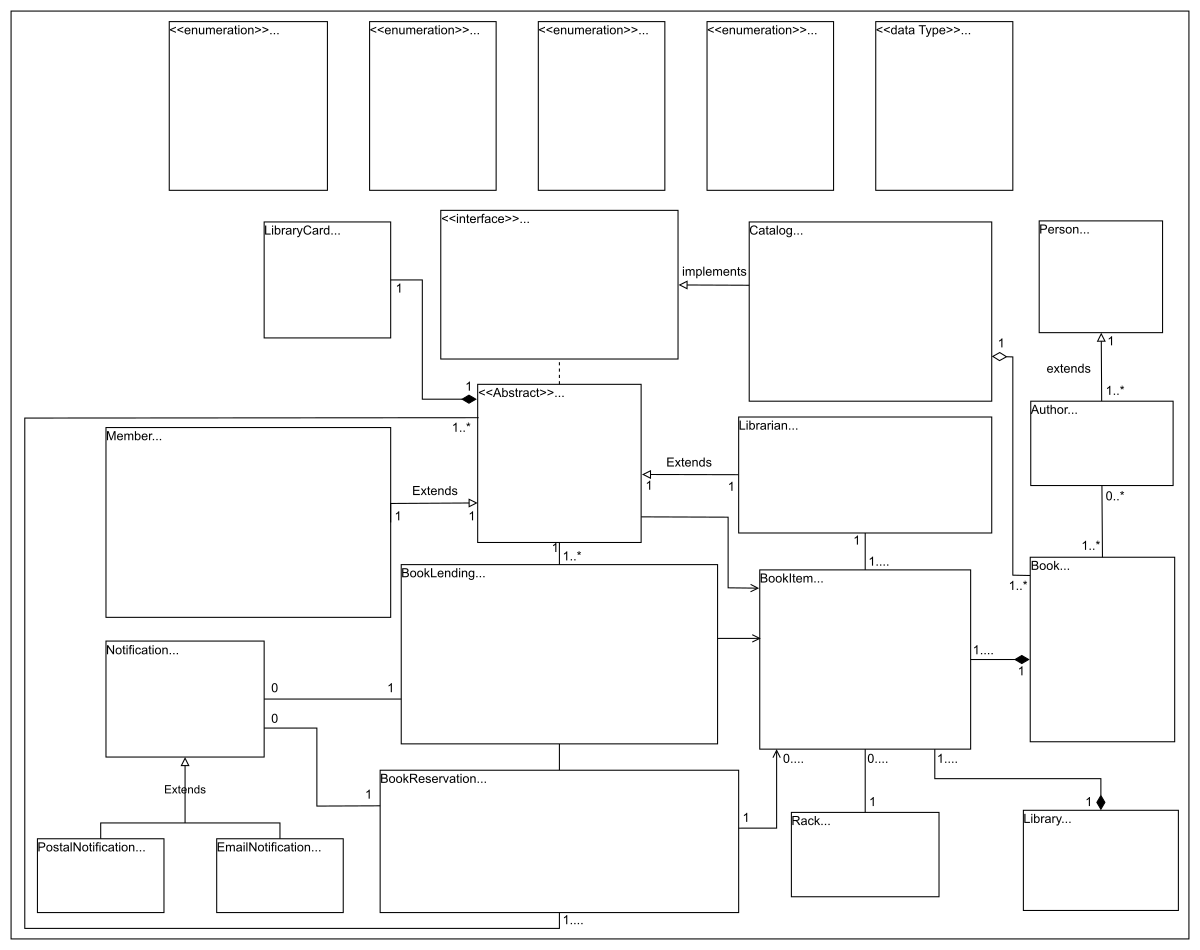
\includegraphics[width=0.5\textwidth]{Images/chapter_9/section_4823331759194112/5793101652033536.png}
 \caption{The class diagram of the library management system}
\end{figure}

\subsection{Design pattern}\label{hMQmE7js8d4-4mpMSx29P}
\\
In our library management system, several well-known object-oriented design patterns are used to ensure the system remains extensible, maintainable, and robust:

\begin{itemize}
\item
\protect\phantomsection\label{z2xf0EbrrGNQKAhZ81fWm}
\textbf{Factory pattern:} We use the Factory pattern to create key domain objects such as \texttt{Book}, \texttt{BookItem}, \texttt{Member}, and \texttt{Librarian} in a consistent and controlled manner. For example, a \texttt{BookFactory} class can encapsulate the logic for creating books with all required metadata and validations. This approach centralizes creation logic, prevents inconsistent states, and supports future extensions such as special editions or new formats.
\item
\protect\phantomsection\label{FKiDKsm-Qsh2Z4X3g18R0}
\textbf{Delegation pattern:} The Delegation pattern helps distribute responsibilities across collaborating classes. For instance, while the \texttt{Librarian} class initiates actions like adding or removing book items, the actual details (such as updating inventory or status) are delegated to the \texttt{BookItem} class. This means \texttt{Librarian} orchestrates, but each \texttt{BookItem} manages its own data and behavior, promoting separation of concerns.
\item
\protect\phantomsection\label{Akp_gGz5KOxihUkc3QBSk}
\textbf{Observer pattern:} The Observer pattern is applied for notification workflows. Members who reserve or are interested in a specific book can be registered as observers. When the status of a \texttt{BookItem} changes (for example, a reserved or unavailable book becomes available), the system automatically notifies all relevant observers (e.g., via email or postal notification). This ensures real-time, event-driven communication and a responsive user experience.
\end{itemize}
\\
These patterns work together to address system complexity, encourage reuse, and make it easier to maintain and extend the system in the future. Later sections and code examples will highlight where these patterns are implemented within the class structure.

\subsection{AI-powered trainer}\label{RETyHp4NJ1-3w2f9vcB6t}
\\
At this stage, everything should be clear. If you encounter any confusion or ambiguity, feel free to utilize the interactive AI-enabled widget below to seek clarification. This tool is designed to help you strengthen your understanding of the concepts.

\begin{figure}[htbp]
 \centering
 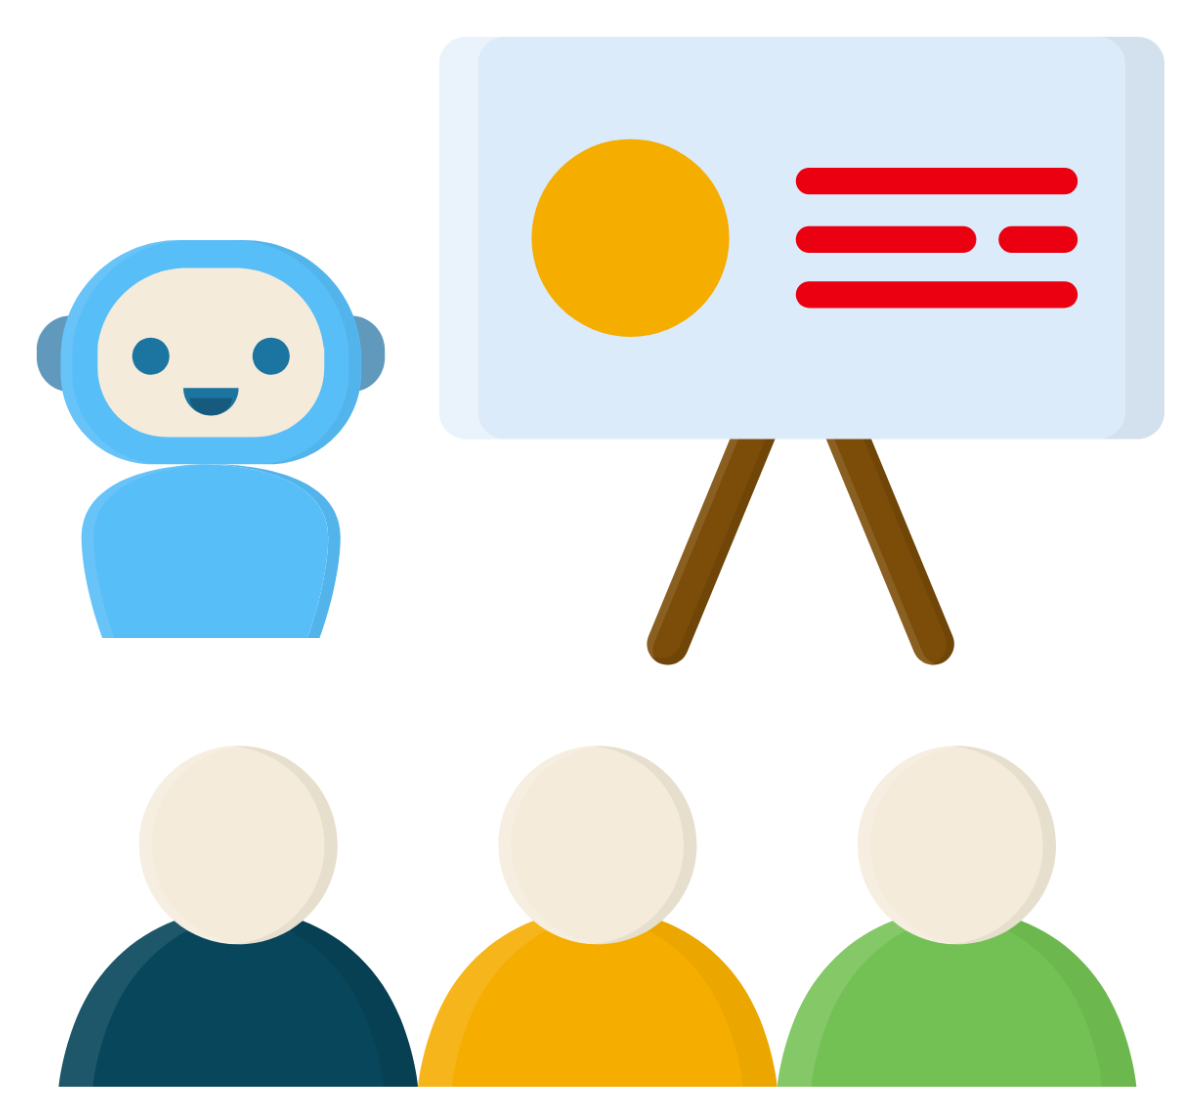
\includegraphics[width=0.15\textwidth]{Images/chapter_9/section_4823331759194112/6604649233514496.png}
 
\end{figure}

\subsection{Additional requirements}\label{NTZYMicWlDqrK06wYITxm}
\\
The interviewer can introduce some additional requirements in the LMS, or they can ask some follow-up questions. Let 's see an example of additional requirements:

% \vspace{-1.0\baselineskip}
\noindent
\begin{minipage}[t]{0.48\textwidth}\vspace{0pt}
\textbf{BarcodeReader:} Each member should have a unique barcode on their library card, and each book should also have a distinct barcode associated with it; the system should be able to scan the barcode of every book and member. To fulfill this requirement, we have the class diagram shown below:
\end{minipage}
\hfill
\begin{minipage}[t]{0.48\textwidth}\vspace{0pt}
\textit{Column component type 'MxGraphWidget' not yet supported.}
\end{minipage}

\begin{figure}[htbp]
 \centering
 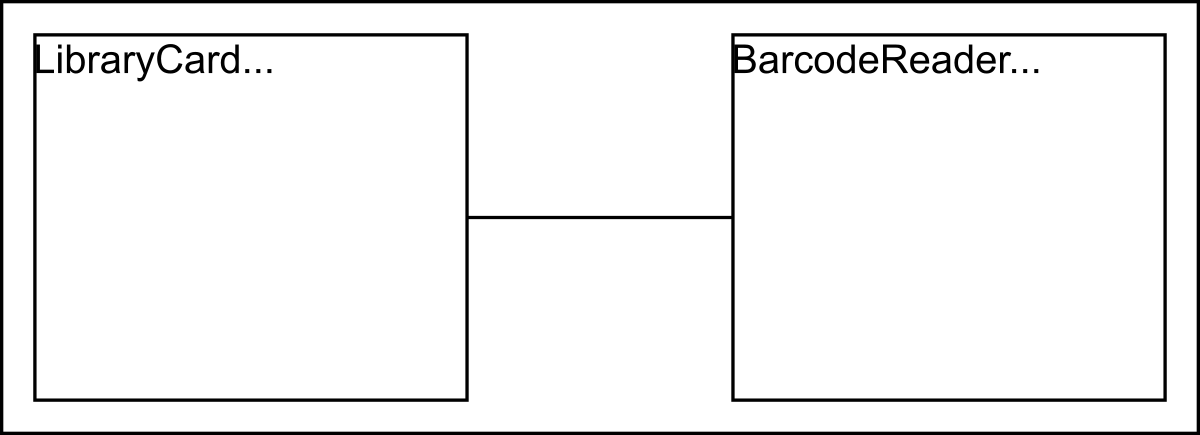
\includegraphics[width=0.5\textwidth]{Images/chapter_9/section_4823331759194112/5760634822852608.png}
 \caption{Relationship between the BarcodeReader and the LibraryCard class}
\end{figure}

% \vspace{-1.0\baselineskip}
\noindent
\begin{minipage}[t]{0.48\textwidth}\vspace{0pt}
\textbf{FineTransaction:} As there is a fine for not returning the book within the time limit, some mechanism should exist to pay the fine. There are three ways to pay the fine: check, cash, or credit card.
\end{minipage}
\hfill
\begin{minipage}[t]{0.48\textwidth}\vspace{0pt}
\textit{Column component type 'MxGraphWidget' not yet supported.}
\end{minipage}

The fine payment functionality follows the \textbf{Decorator pattern} as the fine keeps adding upon the increased number of days. The class diagram provided below shows the relationship of \texttt{FineTransaction} with the \texttt{Fine} class:\\

\begin{figure}[htbp]
 \centering
 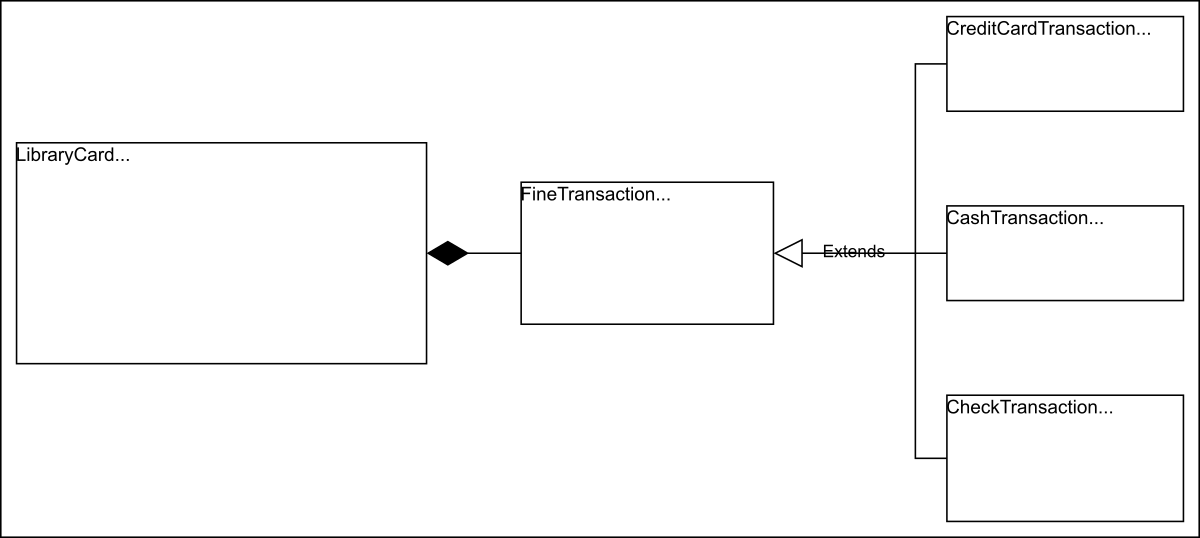
\includegraphics[width=0.5\textwidth]{Images/chapter_9/section_4823331759194112/5554397112434688.png}
 \caption{Relationship of the FineTransaction class with other classes}
\end{figure}

\begin{quote}
\textbf{Quiz:}
\textbf{Question 1:} Let's say that the interviewer asks you what would happen if two or more members try to reserve the same book item. Which member will get the book?
\textbf{Answer:} If two or more members try to reserve the book item at the same time,

the process will be executed on a first come, first serve (FCFS) basis.

For example, the member who comes first gets the book reserved. If two members come simultaneously, the system will check which member has the fewest checked-out books through `totalBooksCheckedOut` and reserve the book item for that particular member. If both members have already reached the maximum number of checkouts, no one can reserve a book.

Note: The member can reserve a book that is currently unavailable, so they will get it first whenever it becomes available.
\end{quote}

We have successfully designed the class diagram for the library management system. Let 's move to the next lesson to see how we can construct the sequence diagram for the system.

% End of section content